% Created 2018-06-21 Thu 12:30
\documentclass[8pt]{beamer}
\usepackage[sc,osf]{mathpazo}   % With old-style figures and real smallcaps.
\linespread{1.025}              % Palatino leads a little more leading
% Euler for math and numbers
\usepackage[euler-digits,small]{eulervm}
%\documentclass[10pt]{llncs}
%\usepackage{llncsdoc}
\usepackage{hyperref}
\usepackage{minted}
\usemintedstyle{xcode}
\usepackage[utf8]{inputenc}
\usepackage[T1]{fontenc}
\usepackage{fixltx2e}
\usepackage{graphicx}
\usepackage{longtable}
\usepackage{float}
\usepackage{wrapfig}
\usepackage{rotating}
\usepackage[normalem]{ulem}
\usepackage{amsmath}
\usepackage{textcomp}
\usepackage{marvosym}
\usepackage{wasysym}
\usepackage{amssymb}
\usepackage{polynom}

\hypersetup{colorlinks=true,
    linkcolor = blue,
    urlcolor  = blue,
    citecolor = blue,
    anchorcolor = blue
}
\renewcommand{\mod}[1]{\left( \texttt{mod}~#1 \right)}
\newcommand{\N}{\mathbb N}
\newcommand{\B}{\mathbb B}
\newcommand{\Z}{\mathbb Z}
\newcommand{\Q}{\mathbb Q}
\newcommand{\C}{\mathbb C}
\newcommand{\degree}{\texttt{degree}}
\newcommand{\cpp}[1]{\mintinline{cpp}{#1}}
\newcommand{\py}[1]{\mintinline{py}{#1}}
\newcommand{\raw}[1]{\mintinline{text}{#1}}
\newcommand{\hs}[1]{\mintinline{hs}{#1}}
\tolerance=1000
\usetheme{Antibes}
% \usetheme{Warsaw}
\author{Siddharth Bhat}
\date{October 18th, 2019}
\institute{IIIT Open Source Developers group}
\title{A taste of Haskell?}
\hypersetup{
  pdfkeywords={},
  pdfsubject={},
  pdfcreator={Emacs 24.5.1 (Org mode 8.2.10)}}
\begin{document}

\maketitle

\begin{frame}[fragile]{What's programming like?}
    A lot like building a cathedral.
    \pause
    \begin{columns}
    \column{0.5\textwidth}
    \begin{figure}
    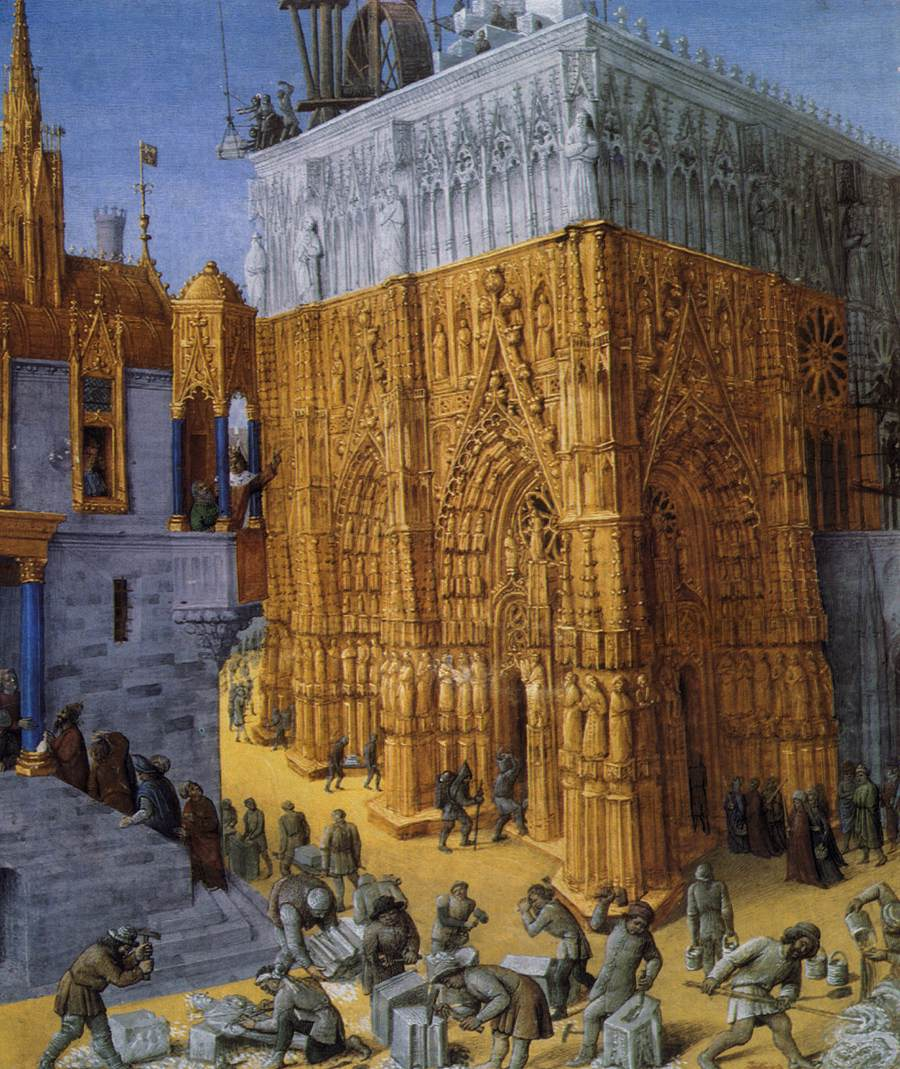
\includegraphics[height=5cm]{./first-we-build.jpg}
    \caption{First we build}
    \end{figure}
    \column{0.5\textwidth}
    \pause
    \begin{figure}
    
\includegraphics[height=5cm]{./then-we-pray.jpg}
    \caption{Then we pray}
    \end{figure}
    \end{columns}
\end{frame}

\begin{frame}[fragile]{Why we pray}
\pause

{\small
\begin{minted}{cpp}
#include <iostream>
#include <climits>
using namespace std;

// f(x) == true ?
bool f(unsigned x) { return (x + 1) > x; }

int main() {
    cout << "f(0): " << f(0) << "\n";
    cout << "f(UINT32_MAX: " << f(UINT32_MAX) << "\n";
}
\end{minted}
}

\pause
\begin{minted}{text}
f(0): 1
f(UINT32_MAX):0
\end{minted}

\pause
\begin{itemize}
    \item 
        $f: \N \rightarrow \B; f(x) \equiv \begin{cases} \texttt{true} & x + 1 > x \\ \texttt{false} & \text{otherwise} \end{cases}$
        \pause
    \item $f(x) \equiv \texttt{true}$ \pause
    \item $f: \N \rightarrow \B; f(x) \equiv \begin{cases} \texttt{true} & x +_{2^{32}} 1 > x \\ \texttt{false} & \text{otherwise} \end{cases}$ \pause
    \item $+_{2^32}: \N \times \N \rightarrow \N; x +_{2^{32}} y \equiv (x +_\N y) \% 2^{32}$ \pause 
    \item $\texttt{UINT32\_MAX} +_{2^{32}} 1 = 0 $
\end{itemize}
\end{frame}


\begin{frame}[fragile]{Why we pray: A second example}
\begin{minted}{cpp}
int main() {
  cout << 2 * ((int) getchar()) << "\n";
}
\end{minted}
\pause

$$ \forall x \in \Z, 2 * x = x + x$$
\pause

\begin{minted}{cpp}
int main() {
  cout << ((int)getchar() + (int)getchar()) << "\n";
}
\end{minted}

\pause


\begin{itemize}
    \item \cpp{int getchar()} \pause
    \item $\texttt{getchar}: \emptyset \rightarrow \texttt{int}$ \pause
    \item $\{ \} \rightarrow \{ 1, 42, \dots \}$ \pause
    \item Such a function can't return an output! \pause
    \item $\texttt{getchar}: \{ \star \} \rightarrow \texttt{int}$ \pause
    \item $\{ \star \} \rightarrow \{ 1, 42, \dots \}$ \pause
    \item $\{ \star \} \rightarrow \{ 1, 42, \dots \}~ \star \mapsto 42$ \pause
    \item Such a function will always return the same output! \pause
    \item \texttt{getchar} can't be a mathematical function.
\end{itemize}

\pause

\end{frame}

\begin{frame}[fragile]{Why we pray: A third example}
\begin{minted}{cpp}
int K (int x, int y) { return x; } // K(x, y) = x
\end{minted}
\pause
\begin{minted}{cpp}
int main() { cout << K(10, 20) << "\n" cout << 10; }
\end{minted}
\pause
\cpp{K(10, 20)} $=  10$
\pause
\begin{minted}{cpp}
int err() { exit(1); return 0; }
int main() { cout << K(10, err()) << "\n" cout << 10; }
\end{minted}
\pause
\cpp{K(10, err())} $\neq 10$
\pause

\begin{itemize}
    \item Mathematically, can replace $K(x, y)$ by $x$. \pause
    \item In C(++), impossible. \pause
    \item cannot \textbf{equationally reason} about programs. \pause
    \item \textbf{Can we} reason about programs? \pause
\end{itemize}
\end{frame}

\begin{frame}[fragile]{Can we reason about C++?}
    \pause
    \begin{itemize}
    \item Short answer: Yes. \pause
    \item Longer answer: Yes. It's complicated. \pause
    \item Name dropping: Operational/Denotational semantics. \pause
    \item Name dropping: Hoare logic/Separation logic. \pause
    \end{itemize}
\end{frame}


\begin{frame}[fragile]{How do we escape having to pray?}
    \pause
    Define a language, \pause where anything that happens, \pause is what \textbf{mathematics} says should happen.
    \pause

\begin{figure}

\includegraphics[height=1cm]{./haskell-logo.png}
\end{figure}
\end{frame}

\begin{frame}[fragile]{A taste of Haskell}
    \begin{itemize}
        \item \hs{let xs = [1, 2,..10]} \pause
        \item \py{xs = range(10)} \pause
        \item \hs{let nats = [1, 2..]} \pause
        \item \py{xs = ??} \pause
        \item \hs{take 2 nats} \pause
        \item \hs{take 10 nats} \pause
        \item \hs{take 100 nats} \pause
        \item Haskell is \emph{lazily evaluated} \pause
    \end{itemize}
\end{frame}

\begin{frame}[fragile]{Why laziness?}
    \begin{itemize}
        \item \hs{let k x y = x} \pause
        \item \hs{k 10 20} \pause
        \item \hs{10 + (error "urk")} \pause
        \item \hs{k 10 (error "urk")} \pause
        \item Laziness provides \emph{equational reasoning}
    \end{itemize}
\end{frame}

\begin{frame}[fragile]{Types}
\begin{itemize}
\item \raw{:t "foo"} \pause
\item \hs{"foo" :: [Char]}
\item \hs{take 2 "foo"} \pause
\item \raw{:t take}
\item \hs{take :: Int -> [a] -> [a]} \pause
\item $\texttt{take} :: \texttt{Int} \rightarrow \texttt{List}(\alpha) \rightarrow \texttt{List}(\alpha)$
\item \hs{take 1 'a'} \pause
\item
\begin{minted}{text}
Prelude> take 1 'a'

<interactive>:11:8: error:
    • Couldn't match expected type ‘[a]’ with actual type ‘Char’
    • In the second argument of ‘take’, namely ‘'a'’
      In the expression: take 1 'a'
      In an equation for ‘it’: it = take 1 'a'
    • Relevant bindings include it :: [a] (bound at <interactive>:11:1)
\end{minted}
\pause
\item If $f: A \rightarrow B$, \pause can ask $f(a)$ for $a \in A$.
\end{itemize}
\end{frame}



\begin{frame}[fragile]{Philosophical differences}

\pause

\begin{columns}% [T] % align columns
\begin{column}{.48\textwidth}
\begin{minted}{py}
" ".join(["a", "b", "c", "d"])
\end{minted}
\pause
\begin{minted}{text}
str.join(iterable)
\end{minted}

Return a string which is the concatenation of the strings in \emph{iterable}. A
\verb|TypeError| will be raised if there are any non-string values in \emph{iterable},
including \verb|bytes objects|. The separator between elements is the string providing
this method.


\end{column}
%
\begin{column}{.48\textwidth}
\pause
\begin{minted}{hs}
intercalate " " ["a", "b", "c", "d"]
\end{minted}

\pause
\begin{minted}{hs}
intercalate :: 
  String -> [String] -> String
intercalate :: 
  [Char] -> [[Char]] -> [Char]
intercalate :: [a] -> [[a]] -> [a]
\end{minted}

\pause
\verb|intercalate xs xss| is \emph{equivalent} to \verb|(concat (intersperse xs xss))|.
It inserts the list \verb|xs| in between the lists in \verb|xss| and concatenates the result.

\pause

\begin{minted}{hs}
intercalate [1, 2] 
  [[3,4], [30, 40], [300, 400]]
\end{minted}

\end{column}
\end{columns}

\pause
{\tiny \url{docs.python.org/3/library/stdtypes.html#str.join}}
{\tiny \url{hackage.haskell.org/package/base-4.14.0.0/docs/Data-List.html#v:intercalate}}

\end{frame}

\begin{frame}[fragile]{Philosophical differences: Abstract algebra}
    \begin{itemize}
        \item Why do we study linear algebra? \pause
        \item Because many things turn out to be linear algebra! \pause
        \item \url{https://math.stackexchange.com/questions/5233/vivid-examples-of-vector-spaces} \pause
        \item Study things at the right level of generality! \pause
        \item Words Words: Monoids, Groups, Rings, Fields, Partial orders, Lattices, \dots \pause
        \item \raw{str.join(iterable)} versus \hs{intercalate :: [a] -> [[a]] -> [a]} \pause
        \item What is an iterable anyway? \pause
    \end{itemize}
\end{frame}

\begin{frame}[fragile]{Summing over a list of numbers}


\begin{columns}% [T] % align columns
\begin{column}{.48\textwidth}
\begin{minted}{py}
sum([1, 2, 3, 4])
\end{minted}
\pause
\begin{minted}{text}
sum(iterable, /, start=0)
\end{minted}

Sums \emph{start} and the items of an \emph{iterable} from left to right and
returns the total. The \emph{iterable}’s items are normally numbers, and the start
value is not allowed to be a string.

\pause

\end{column}
%
\begin{column}{.48\textwidth}
\begin{minted}{hs}
sum [1, 2, 3, 4]
\end{minted}

\pause
\begin{minted}{hs}
sum :: (Foldable t, Num a) => t a -> a
sum :: [Int] -> Int]
\end{minted}
\pause
The \verb|sum| function computes the sum of the numbers of a structure.

\end{column}
\end{columns}

\pause
\begin{itemize}
    \item \hs{sum [1, 2, 3]} \pause
    \item \hs{sum [1.1, 2.1, -3.2]} \pause
    \item \hs{let minus_1_by_12 = sum [1, 2..]}
\end{itemize}

\pause

{\tiny \url{https://docs.python.org/3/library/functions.html#sum}}
{\tiny \url{hackage.haskell.org/package/base-4.14.0.0/docs/Data-List.html#v:intercalate}}

\end{frame}

\begin{frame}[fragile]{\texttt{Num}?}
\hs{sum :: (Foldable t, Num a) => t a -> a}

\pause
\begin{minted}{hs}
class  Num a  where -- Typeclass: `a` is a Num if...
\end{minted}
\pause
\begin{minted}{hs}
    (+), (-), (*)       :: a -> a -> a
\end{minted}
\pause
\begin{minted}{hs}
    -- | Unary negation.
    negate              :: a -> a
    -- | Absolute value.
    abs                 :: a -> a
\end{minted}
\pause
\begin{minted}{py}
    -- | Sign of a number.
    -- The functions 'abs' and 'signum' should satisfy the law:
    --
    -- > abs x * signum x == x
    --
    -- For real numbers, the 'signum' is either `-1` (negative), `0` (zero)
    -- or `1` (positive).
    ...
\end{minted}

\pause
\begin{itemize}
    \item Associativity of \raw{+} \raw{(x + y) + z = x + (y + z)} \pause
    \item Commutativity of \raw{+}: \raw{x + y = y + x} \pause
    \item \raw{negate} gives the additive inverse: \raw{x + negate x = fromInteger 0} \pause
\end{itemize}

\pause
\url{https://hackage.haskell.org/package/base-4.14.0.0/docs/Prelude.html#t:Num}

\end{frame}

\begin{frame}[fragile]{\texttt{Foldable}?}

A thing one can accumulate answers on. So a list, a set, a binary tree, \dots

\begin{itemize}
    \item \hs{let x = Data.Set.fromList [1, 2, 3]} \pause
    \item \hs{fromList [1,2,3]} \pause
    \item \hs{let y = union x x} \pause
    \item \raw{fromList [1,2,3]} \pause
    \item \hs{sum y}
    \item \raw{6}
\end{itemize}
\end{frame}

\begin{frame}[fragile]{\texttt{Foldable} in detail}


\begin{minted}{hs}
class Foldable t where
  -- | Map each element of the structure to a monoid, and combine the results.
  foldMap :: Monoid m => (a -> m) -> t a -> m
\end{minted}

\verb|Foldable| instances are expected to satisfy the following laws:

\begin{minted}{hs}
foldr f z t = appEndo (foldMap (Endo . f) t ) z
foldl f z t = appEndo (getDual (foldMap (Dual . Endo . flip f) t)) z
fold = foldMap id
length = getSum . foldMap (Sum . const  1)
\end{minted}
{\tiny \url{https://hackage.haskell.org/package/base-4.14.0.0/docs/Data-Foldable.html#t:Foldable}}
\end{frame}

\begin{frame}[fragile]{Should I learn hasell?}

\begin{itemize}
\item Will it help me get a job? \pause Unlikely \pause
\item Will it help me do better at CP? \pause Ask Anurudh \pause
\item Will it help me get a GSoC project? \pause Maybe. The haskell community is small! \pause
\item Will it help me learn math? \pause Yes. \pause
\item Will it help me \textbf{understand what computation is}? \pause Yes. It was designed to do so \pause
\end{itemize}

\pause
\begin{quote}
    The Haskell motto: Avoid success at all costs
\end{quote}
\pause
\begin{quote}
    The Haskell motto: Avoid success\textcolor{red}{,} at all costs
\end{quote}
\pause
\begin{quote}
    The Haskell motto: Avoid \textcolor{blue}{``} success at all costs \textcolor{blue}{''}
\end{quote}
\end{frame}

\begin{frame}[fragile]{The end: What is haskell?}
    \begin{itemize}
        \item Haskell is a programming language \pause
        \item It is lazy: \hs{k 10 (error "urk")} \pause
        \item It is strongly typed: \hs{take :: Int -> [a] -> [a]}\pause
        \item It is pure (We didn't talk about this)\pause
        \item Its community is fanatical \pause \dots  about having the right abstractions: \hs{Foldable}, \hs{Num} \pause
    \end{itemize}
    Where to learn?
    \begin{itemize}
        \item The Freenode IRC channel \raw{##haskell}\pause
        \item \href{https://www.seas.upenn.edu/~cis194/fall16/}{CIS 194: Introduction to Haskell (course at UPenn)} \pause
        \item \href{http://learnyouahaskell.com/}{The book \raw{learn you a Haskell for great good}} \pause
        \item In-house: Watch anurudh solve CP problems in Haskell\pause
        \item In-house: 
            \href{https://discord.com/invite/zK3a9n6?fbclid=IwAR1JaASmpgyc7T8w49E2aE-hr58ppwlr7QuZBK8Ssdk6Un9eXHYwUPm93-g}{Ping folks in the Theory group with questions}\pause
    \item In-house: DM me with questions, or \href{https://calendly.com/bollu/}{Pick a time to chat with me} \pause
    \end{itemize}
\end{frame}


\begin{frame}[fragile]{Dictionary ordering}
\begin{quote}
Oh, that's just monoidal accumulation of a left absorbing semigroup
\end{quote}
\end{frame}


\begin{frame}[fragile]{Fibonacci, Take 1}
\begin{itemize}
    \item \hs{fib :: Int -> Int}. Produces $n$th fibonacci number
    \item \hs{fib 0 = 0}\pause
    \item \hs{fib 1 = 1}\pause
    \item \hs{fib n = fib (n - 1) + fib (n - 2)}\pause
    \item \hs{fibs :: [Int]} \pause
    \item \hs{fib = ???}\pause
    \item Empty list: \hs{[]} \pause
    \item append an element using \hs{:} --- \hs{[1] = 1:[]}\pause
    \item append an element using \hs{:} --- \hs{[1, 2] = 1:2:[]}\pause
    \item append an element using \hs{:} --- \hs{[1, 2, 3] = 1:2:3:[]}\pause
    \item Convert a list \hs{[0, 1, 2...]} into a list \hs{[fib 0, fib 1, fib 2, ...]}
\end{itemize}

\pause

\begin{itemize}
    \item \hs{ys = map f xs}
    \item \hs{xs=[x1, x2 ... xn]} $\implies$
    \item \hs{[f x1, f x2, ..., f xn] = ys}
    \item \hs{fibs = map fib [0, 1..]} \pause
    \item \hs{map [] = []} \pause; \hs{map (x:xs) = (f x):(map f xs)}\pause
    \item \hs{map :: (t1 -> t2) -> [t1] -> [t2]}
\end{itemize}
\pause
\end{frame}

\begin{frame}[fragile]{Fibonacci, Take 2}
\begin{itemize}
    \item \hs{fibs} satisfies a recurrence:
    \item \hs{fibs ! 0 = 0}
    \item \hs{fibs ! 1 = 1}
    \item \hs{fibs ! n = fibs ! (n - 1) + fibs ! (n - 2)}
\end{itemize}
\pause

\begin{minted}{raw}
fibs = [0, 1, ?]
              1
            + 0
            = 1
\end{minted}
\pause
\begin{minted}{raw}
fibs = [0, 1, 1, ?]
                 1
               + 1
               = 2
\end{minted}
\pause
\begin{minted}{raw}
[fib 0, fib 1, fib 2, fib 3, fib 4, ..., fib (n-1), fib n]  
[fib 1, fib 2, fib 3, fib 4, fib 5, ..., fib (n-2), fib (n-1)]
=
[fib 2, fib 3, fib 4, fib 5, fib 6, ..., fib  n   , fib (n+1)]

\begin{minted}{raw}
zipWith f xs ys

[x1, x2, x3 ... xn]
  f  f   f      f   => [f x1 y1, f x2 y2, ..., f xn yn
[y1, y2, y3 ... yn]
\end{minted}
\pause
\begin{minted}{hs}
zipWith (<>) ["how ", "hello "] ["are you?", "world!", "extra"] ==
 ["how are you?", "hello world!"]
\end{minted}
\pause
\begin{minted}{hs}
zipWith f [] [] = []
zipWith f (x:xs) [] = []
zipWith f (x:xs) (y:ys) = (f x y):zipWith xs ys
\end{minted}
\pause

\begin{minted}{hs}
let fibs = 0:1:(zipWith (+) fibs (tail fibs))
\end{minted}
\end{frame}

\begin{frame}[fragile]{IO in haskell}
\begin{itemize}
    \item \cpp{int getchar()} \pause
    \item \hs{getChar :: IO Char} \pause
    \item \hs{(*) :: Int -> Char -> Int} \pause
    \item \hs{1 * getChar -- does not typecheck} \pause
    \item \hs{do x <- getChar; print (2 * (fromEnum x))} \pause
    \item \hs{  x :: Char} because \hs{getChar :: IO Char}
    \item \hs{2 * (fromEnum x) == fromEnum x + fromEnum x}\pause
    \item \cpp{int x = getchar(); 2 * x == x + x}\pause
    \item \cpp{2 * getchar() != getchar() + getchar()}
\end{itemize}
\end{frame}

\begin{frame}[fragile]{Effects, or the ``\texttt{M}'' word}
Keep every element, and drop every element.
\begin{minted}{hs}
powerset xs = filterM (const [True, False]) xs
\end{minted}
\end{frame}

\begin{frame}[fragile]{Currying}
\begin{itemize}
\item \hs {let peek x = take 1 x} \pause
\item \hs {let peek'= take 1} \pause
\item \hs {peek' x = take 1 x} \pause
\item Equational reasoning! \pause
\item \hs{let x_incr = 1 + x} \pause
\item \hs{let x_incr = (+) 1 x} \pause
\item \hs{let incr = (+) 1} \pause
\end{itemize}
\end{frame}

\begin{frame}[fragile]{Trolling the Haskell IRC channel}
{\tiny \url{https://gist.githubusercontent.com/quchen/5280339/raw/a18362f99e3847351e891f2ed37872d1dfa9f942/trolling_haskell}}
{\tiny
\begin{minted}{raw}
xQuasar>      | HASKELL IS FOR FUCKIN FAGGOTS. YOU'RE ALL A BUNCH OF 
              | FUCKIN PUSSIES
xQuasar>      | JAVASCRIPT FOR LIFE FAGS
luite>        | hello
ChongLi>      | somebody has a mental illness!
merijn>       | Wow...I suddenly see the error of my ways and feel 
              | compelled to write Node.js!
genisage>     | hi
luite>        | you might be pleased to learn that you can compile 
              | haskell to javascript now
xQuasar>      | FUCK YOU AND YOUR HUSSY OPS
xQuasar>      | THEY CAN'T DO SHIT TO ME CUNTS
quchen>       | xQuasar: While I don't think anything is wrong with 
              | faggots to the point where "faggot" isn't insulting 
              | anymore, I assure you we have heterosexuals in our 
              | language as well.
quchen>       | Haskell is invariant under gender. Really!
Iceland_jack> | quchen++
merijn>       | I don't blame him, I'd be this angry to if I had to write 
              | javascript all day too
xQuasar>      | FUCK YOU STRAIGHT CUNTS
xQuasar>      | BESTIALITY IS THE BEST
quchen>       | merijn: Lol. And when I write that I mean it :D
quchen>       | xQuasar: Do you have any specific questions?
merijn>       | This is sort of like a puppy trying to be angry with 
              | you...it's just kinda adorable to see him think he has 
              | any effect :)
quchen>       | xQuasar: You're offtopic right now. This is a Haskell 
              | help channel. Do you have Haskell questions?
quchen>       | xQuasar: We'd love to help you make your first steps.
tsinnema>     | hey -- is there a proper way to whine about no one having
              | responded to a question? :)
xQuasar>      | i just want to get kicked out of a bunch of channels for 
              | fun
quchen>       | Have you seen LYAH? It's a very enjoyable book on 
              | Haskell. It also has a reputation of being very 
              | uplifting.
\end{minted}
}
\end{frame}

\begin{frame}[fragile]{Trolling the Haskell IRC channel}
{\tiny \url{https://gist.githubusercontent.com/quchen/5280339/raw/a18362f99e3847351e891f2ed37872d1dfa9f942/trolling_haskell}}
{\tiny
\begin{minted}{raw}
quchen>       | @where lyah
xQuasar>      | why is no one cooperating with me
lambdabot>    | http://www.learnyouahaskell.com/
tsinnema>     | in soviet russia, haskell learns a you
merijn>       | tsinnema: Yeah, wait 30 minutes or more and try again :)
Iceland_jack> | xQuasar: We are cooperating with you, you're just not 
              | aware that your goal is learning Haskell
ChongLi>      | xQuasar: why not learn some Haskell instead?
xQuasar>      | alright i'll admit i lose
merijn>       | Ha, sometimes I forget how hard it is to troll haskell :)
nxorg8>       | #haskell is awesome :-)
xQuasar>      | what's haskell good for though
quchen>       | xQuasar: But there is so much to win here!
xQuasar>      | i'm more into gamedev
Iceland_jack> | figures
arkeet>       | it's good for writing programs.
xQuasar>      | what kind of programs?
ChongLi>      | xQuasar: any kind
arkeet>       | "what's C++ good for?"
Iceland_jack> | xQuasar: The ones that run on comput-ars.
ChongLi>      | it's a general purpose language
luite>        | xQuasar: frp can be useful for writing games, and with 
              | ghcjs you can compile them to javascript to make web 
              | games
tsinnema>     | merijn, yeah, seems reasonable :)
ChongLi>      | seriously though, if you learn it you may completely 
              | change your perspective on programming
xQuasar>      | i have absolutely no idea what frp and ghcjs are
...
\end{minted}
}
\end{frame}


\begin{frame}{Equality}
\end{frame}

\end{document}
